\documentclass[11pt,a4paper]{article}
\usepackage[margin=0.9in]{geometry}
\usepackage{amsmath,amssymb,amsthm,mathtools,bm}
\usepackage{booktabs,array,longtable,tabularx}
\usepackage{enumitem,xcolor,tikz}
\usetikzlibrary{positioning,arrows.meta}
\usepackage{hyperref}
\definecolor{ink}{HTML}{112F43}
\definecolor{teal}{HTML}{087F82}
\definecolor{coral}{HTML}{CB5D4D}
\hypersetup{colorlinks=true,linkcolor=teal,citecolor=teal,urlcolor=teal,pdftitle={Understanding d-LIN through ABW09}}
\setlength{\parskip}{0.45em}
\setlength{\parindent}{0pt}
\setlength{\emergencystretch}{2em}
\setlist{topsep=3pt,itemsep=3pt,leftmargin=*}
\setlist[description]{style=nextline,leftmargin=0pt,labelindent=0pt,labelwidth=0pt,labelsep=0pt}
\newcolumntype{Y}{>{\raggedright\arraybackslash}X}
\newcommand{\F}{\mathbb F}
\newcommand{\Z}{\mathbb Z}
\newcommand{\E}{\mathbb E}
\newcommand{\wt}{\operatorname{wt}}
\newcommand{\Image}{\operatorname{Im}}
\newcommand{\Ber}{\operatorname{Ber}}
\newcommand{\Bin}{\operatorname{Bin}}
\newcommand{\Search}{\operatorname{Search3LIN}}
\newcommand{\App}{\operatorname{AppSearch3LIN}}
\newcommand{\Predict}{\operatorname{Predict3LIN}}
\newcommand{\Decide}{\operatorname{Decide3LIN}}
\newcommand{\cM}{\mathcal M}
\newcommand{\one}{\mathbf 1}
\newcommand{\zero}{\mathbf 0}
\newcommand{\readref}[1]{\textcolor{teal}{\small\textbf{Paper reference:} #1}}
\newtheorem{observation}{Observation}
\title{\textbf{Understanding d-LIN through ABW09}\\[5pt]
\large Problem definitions, hardness assumptions, comparisons,\\and public-key cryptography}
\author{Prajjwal Saxena\\\small Revised with the assistance of GPT}
\date{5 October 2026}

\begin{document}
\maketitle
\begin{abstract}
The $d$-LIN setting studied by Applebaum, Barak and Wigderson (ABW) consists of random sparse binary equations with independently flipped outputs. These notes explain what is sampled, what an attacker is asked to compute, and which assumptions lead to public-key encryption. They then compare this setting with LPN, LWE and Module-LWE. The main distinction is between a simple algebraic decryption identity and a complete security argument: a short hidden dependency enables decryption, but the distribution of the public key, the noise parameters and the reduction are essential. ABW's result establishes a conditional theoretical foundation, rather than a concrete modern encryption standard.
\end{abstract}

\textbf{Source and scope.} ``ABW09'' means the supplied 57-page manuscript dated 7 November 2009, \emph{Public-Key Cryptography from Different Assumptions} \cite{abw}. Section, theorem and printed-page references below refer to that manuscript, whose numbering differs from shorter versions. Contemporary comparisons use the additional primary sources in the bibliography. Calculations and teaching examples are identified separately from paper results.

\textbf{Reading paths.} For a first reading, follow Sections~\ref{sec:model}--\ref{sec:noise}, the opening paragraphs of Section~\ref{sec:tasks}, and Sections~\ref{sec:pke}, \ref{sec:compare}, and \ref{sec:assessment}. For a seminar, also study the exact assumptions and reduction discussion in Sections~\ref{sec:assumptions} and \ref{sec:evidence}. The final exercises check the distinctions most likely to cause confusion.
\tableofcontents
\newpage

\section{The sampled problem}\label{sec:model}
\subsection{Bits, dimensions and local equations}
All operations in the $d$-LIN model use the binary field $\F_2=\{0,1\}$. Addition is XOR: $1+1=0$, and subtraction equals addition. A clause is a parity equation involving exactly $d$ distinct variables. For example,
\[
 x_1+x_2+x_4=b_i
\]
has row vector $(1,1,0,1,0)$ and row weight three.

The sampled observation is
\begin{equation}\boxed{b=Mx+e\quad\text{over }\F_2.}\label{eq:model}\end{equation}
The full dimensions, including column-vector representations, are
\begin{equation}
 M\in\F_2^{m\times n},\qquad
 b=\begin{pmatrix}b_1\\b_2\\\vdots\\b_m\end{pmatrix},\quad
 x=\begin{pmatrix}x_1\\x_2\\\vdots\\x_n\end{pmatrix},\quad
 e=\begin{pmatrix}e_1\\e_2\\\vdots\\e_m\end{pmatrix}.
\end{equation}
Here $m$ counts equations, $n$ counts variables and $d$ counts selected variables per equation. In the inference problem, the observer receives $(M,b)$, while $x$ and $e$ are hidden.

\subsection{The distribution is part of the definition}
The ensemble $\cM_{m,n,d}$ selects each row independently and uniformly from the $\binom nd$ binary vectors of weight $d$. A variable can appear in many rows; column weights are not fixed. Different rows can repeat. Sampling proceeds as follows:
\begin{align}
 M&\leftarrow\cM_{m,n,d}, &x&\leftarrow\operatorname{Uniform}(\F_2^n),\\
 e_i&\overset{\mathrm{iid}}\sim\Ber(\epsilon),&b&=Mx+e.
\end{align}
The three random choices are independent. Usually $0<\epsilon<1/2$. In an asymptotic claim, $m$, $d$ and $\epsilon$ may depend on $n$; ABW's main linear constructions use constant locality.

An arbitrary sparse matrix is not a sample from this ensemble. In particular, a matrix sampled together with a secret dependency has a special key-generation distribution. The proof must relate that distribution to the random ensemble on which hardness is assumed.

\readref{ABW Section 4, printed p.~11; Definition 5.1, p.~12.}

\subsection{A factor-graph view}
One can represent each equation by a square and each variable by a circle. An edge means that the variable occurs in that equation. The following graph encodes the example in Section~\ref{sec:example}; the second observed output is the flipped one.
\begin{center}
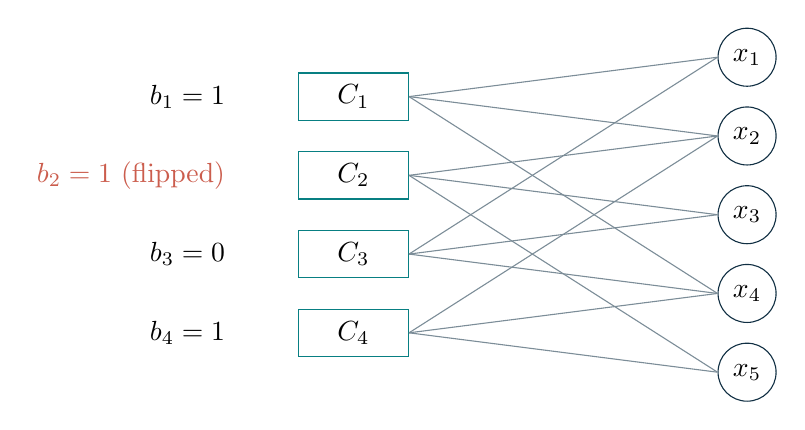
\begin{tikzpicture}[x=1cm,y=1cm,eqn/.style={draw=teal,rectangle,minimum width=1.4cm,minimum height=.6cm},var/.style={draw=ink,circle,minimum size=.55cm}]
\foreach \i/\y in {1/3,2/2,3/1,4/0}{\node[eqn] (c\i) at (0,\y) {$C_{\i}$};}
\foreach \j/\y in {1/3.5,2/2.5,3/1.5,4/.5,5/-.5}{\node[var] (x\j) at (5,\y) {$x_{\j}$};}
\foreach \i/\j in {1/1,1/2,1/4,2/2,2/3,2/5,3/1,3/3,3/4,4/2,4/4,4/5}{\draw[ink!55] (c\i.east)--(x\j.west);}
\node[left=8mm of c1] {$b_1=1$};\node[left=8mm of c2,text=coral] {$b_2=1$ (flipped)};
\node[left=8mm of c3] {$b_3=0$};\node[left=8mm of c4] {$b_4=1$};
\end{tikzpicture}
\end{center}
Each square has degree three. The picture makes locality visible; it does not establish computational hardness.

\section{An example and the geometry of errors}\label{sec:example}
Take the same matrix and column vectors used in the original notes:
\begin{equation}
 M=\begin{pmatrix}1&1&0&1&0\\0&1&1&0&1\\1&0&1&1&0\\0&1&0&1&1\end{pmatrix},\quad
 x=\begin{pmatrix}1\\0\\1\\0\\1\end{pmatrix},\quad
 e=\begin{pmatrix}0\\1\\0\\0\end{pmatrix}.
\end{equation}
Multiplication and addition over $\F_2$ give
\begin{equation}
 Mx=\begin{pmatrix}1\\0\\0\\1\end{pmatrix},\qquad
 b=Mx+e=\begin{pmatrix}1\\1\\0\\1\end{pmatrix}.
\end{equation}
For any candidate $z$, its residual $Mz-b$ records the violated clauses. Hamming weight $\wt(v)$ counts the ones in a binary vector, so
\begin{equation}
 \text{fraction of clauses satisfied by }z=1-\frac{\wt(Mz-b)}m.
\end{equation}
The planted $x$ has one violation and satisfies $3/4$ of these four clauses. However,
\[
 x'=\begin{pmatrix}0\\1\\0\\0\\0\end{pmatrix}\qquad\text{satisfies}\qquad Mx'=b.
\]
Thus this toy instance is fully satisfiable despite the sampled error. Its row rank is four, so $\Image(M)=\F_2^4$. The example demonstrates arithmetic, not hardness or unique recovery.

\subsection{Distance to one codeword versus the whole image}
The image $C=\Image(M)=\{Mz:z\in\F_2^n\}$ is a binary linear code. The sampling procedure picks a codeword $Mx$ and adds $e$. Consequently,
\begin{align}
 d_H(b,Mx)&=\wt(e),\\
 d_H(b,C)&=\min_z\wt(b-Mz)\leq\wt(e).\label{eq:distance}
\end{align}
The first distance is to the particular planted output. The second is to the nearest codeword and can be strictly smaller, as the example shows. Therefore
\[
 \E[d_H(b,Mx)]=m\epsilon,\qquad \E[d_H(b,C)]\leq m\epsilon.
\]
The inequality should not be replaced by a general equality. This also separates three possible goals: recovering the planted secret, recovering its clean codeword and finding any closest codeword.

\section{What the noise parameter means}\label{sec:noise}
\subsection{A random error count is not a deterministic cap}
Let $W=\wt(e)$. Independent Bernoulli noise gives
\begin{equation}
 W\sim\Bin(m,\epsilon),\quad
 \Pr[W=k]=\binom mk\epsilon^k(1-\epsilon)^{m-k},\quad 0\leq k\leq m.
\end{equation}
Its mean and variance are
\begin{equation}\E[W]=m\epsilon,\qquad\operatorname{Var}(W)=m\epsilon(1-\epsilon).\end{equation}
For $t>0$, Hoeffding's inequality gives the useful upper-tail bound
\begin{equation}\Pr[W/m>\epsilon+t]\leq\exp(-2mt^2).\label{eq:hoeffding}\end{equation}
These are direct calculations for the model, not additional hardness assumptions.

By contrast, an instance is \emph{$(1-\rho)$-satisfiable} if some assignment $z$ obeys the deterministic bound $\wt(Mz-b)\leq\rho m$. We use $\rho$ for this bound to keep it distinct from the sampling probability $\epsilon$. Equation~\eqref{eq:hoeffding} says that a sampled instance is $(1-\epsilon-t)$-satisfiable with probability at least $1-\exp(-2mt^2)$, using the planted $x$ as a witness. Sampling does not guarantee $W\leq m\epsilon$.

\subsection{Interpreting the requested examples}
For the graphs with $m=20$, the exact moments are
\begin{center}
\begin{tabular}{ccc}\toprule
$\epsilon$ & $\E[W]$ & $\operatorname{Var}(W)$\\\midrule
0.50 &10&5\\0.25&5&3.75\\0.70&14&4.2\\\bottomrule
\end{tabular}
\end{center}
These distributions illustrate noise; they are not ABW parameter recommendations.
\begin{itemize}
\item At $\epsilon=1/2$, $e$ is uniform, so $b$ is uniform and independent of $x$, even after fixing $M$. Exact recovery then fails for an information-theoretic reason. This setting also destroys the parity bias needed for ABW decryption.
\item At a known $\epsilon>1/2$, replace $b$ by $b+\one_m$. The new error is $e+\one_m\sim\Ber(1-\epsilon)^m$. Hence $0.7$ is equivalent to $0.3$ after relabeling; it does not simply provide stronger security than $0.5$.
\item At $\epsilon=0$, an exact system can be solved by Gaussian elimination. Some solutions may be nonunique, but finding one is efficient.
\end{itemize}

\section{The computational tasks}\label{sec:tasks}
The equation alone does not specify a computational problem. The goal, distribution and success criterion must also be stated.

\subsection{Planted search and approximate recovery}
ABW Definition 5.1 defines $\Search(m,\epsilon)$ by the sampling experiment above with $d=3$, and asks for the planted $x$. Intractability means that every probabilistic polynomial-time (PPT) algorithm has recovery probability less than $2/3$ for all sufficiently large $n$.

ABW Definition 6.1 defines $\App(m,\epsilon)$ by asking for $\widehat x$ with
\[
 d_H(\widehat x,x)\leq0.1n.
\]
The stated intractability threshold there is success probability $0.7$. This is proximity to the \emph{secret}, not merely a bound on $\wt(M\widehat x-b)$. Good fitting and good recovery need separate justification before being interchanged.

\subsection{Decision and prediction}
The decision problem compares
\begin{align}
 \mathcal D_{\rm noisy}&=(M,Mx+e),\\
 \mathcal D_{\rm random}&=(M,u),\qquad u\leftarrow\operatorname{Uniform}(\F_2^m),
\end{align}
with the same matrix law in both experiments and all random choices independent. A distinguisher $A$ has advantage
\[
 \left|\Pr[A(\mathcal D_{\rm noisy})=1]-\Pr[A(\mathcal D_{\rm random})=1]\right|.
\]
The prediction problem instead asks for $\langle v,x\rangle$ from noisy equations and a further sparse row $v$. The distribution of the existing rows together with $v$ matters. Predicting this clean parity is central to the encryption proof.

\subsection{Optimization and refutation}
Nearest-codeword optimization asks to minimize $\wt(Mz-b)$ over $z$. Refutation asks for a certificate that an instance cannot satisfy a specified fraction of its clauses. These are useful related questions, but neither is interchangeable with planted recovery by definition. Worst-case NP-hardness of a related optimization problem does not establish average-case cryptographic hardness for a sampled ensemble.

\subsection{Identifiability and the parity of locality}
If $\ker M\ne\{0\}$, the observation law is identical for secrets that differ by a kernel vector. In particular, when every row has even weight,
\[
 M\one_n=\zero_m,\qquad M(x+\one_n)=Mx.
\]
Unique recovery of the literal planted $x$ is then impossible without a convention or extra information. A generalized search task should specify recovery up to this symmetry, recovery of $Mx$, or an equivalent normalization. These are mathematical qualifications, not a silent redefinition of ABW's exact 3-LIN task. For a clean reading of the linear constructions, the locality-three search problem and locality-six public-key route avoid confusing an even public-matrix degree with the degree of the assumed search problem.

\readref{ABW Sections 5.1 and 6.1--6.2, printed pp.~12--18.}

\section{The hardness assumptions and theorems}\label{sec:assumptions}
\subsection{The 3-LIN-only route}
ABW Assumption 5.2 asserts that, for positive constants $C_0,C_1$,
\begin{equation}
 \Search(C_0 n^{1.4},C_1 n^{-0.2})\quad\text{is intractable.}\label{eq:assumption}
\end{equation}
The paper states this for every positive choice of the constants; footnote 9 explains that its applications need only particular universal constants from the reductions. Theorem 2 summarizes the result as follows: there is a constant $c$ such that hardness at $m=cn^{1.4}$ and $\epsilon=n^{-0.2}/c$ implies semantically secure public-key encryption. Corollary 5.6 gives the detailed conclusion.

This is an \emph{average-case}, parameter-specific assumption against PPT algorithms. The claim is not that every sparse noisy instance is hard, or that a $2^n$ search space proves exponential complexity. Noiseless linear algebra already illustrates why a large candidate space need not imply a slow algorithm.

\subsection{The d-LIN plus expansion route}
Theorem 3 uses a lower-density search regime together with an additional assumption. To avoid overloading symbols, use $d_s$ for search locality and $Q$ for the size of a planted shrinking set. Its overview has the form
\begin{equation}
 \begin{gathered}
 d_s\text{-LIN}(c'n\log n,1/(c'Q))\quad\text{and}\quad
 \operatorname{DUE}(cn,Q,2d_s)\\
 \Longrightarrow\quad\text{semantically secure PKE},
 \end{gathered}\label{eq:dueoverview}
\end{equation}
under the paper's admissible parameter conditions. Here the DUE notation lists graph row count, planted-set size and degree, as in the introduction. The detailed Section 7 writes its arguments in a different order.

DUE, \emph{Decisional Unbalanced Expansion}, compares a random bipartite graph with a graph in which $Q$ selected equation vertices are rewired to only $Q/3$ variable vertices. Each equation vertex still has the prescribed degree. The hypothesis is that efficient algorithms cannot distinguish these graph distributions with the stated advantage.

In the detailed Assumption 7.2, write $D=2d_s$ for the even public-matrix locality. There must be a function $Q=o(n)$ and a suitable constant $D$ for which:
\begin{enumerate}
\item $\operatorname{SearchLIN}(D/2,m_S,\eta)$ is intractable for every $m_S=O(n\log n)$ and $\eta=\Omega(1/Q)$ in the stated regime;
\item $\operatorname{DUE}(D,Cn,Q)$ is $1/(2000C^2)$-intractable for sufficiently large constant $C$, using Section 7's argument order.
\end{enumerate}
The public-key graph has $\Theta(n)$ rows in Corollary 7.5, whereas the search reduction uses $O(n\log n)$ samples. Do not identify these two counts. The paper discusses $Q=n^\delta$ for suitably small positive $\delta$, such as $1/10$, with restrictive constant choices. These are asymptotic examples, not concrete security levels.

\subsection{A parameter conversion that matters}
The Section 7 reduction pairs noisy equations. XOR of two independent $\Ber(\eta)$ bits is $\Ber(2\eta(1-\eta))$. Thus Theorem 7.3 relates ciphertext locality $D$ and error rate $\epsilon$ to search locality $D/2$ and rate
\begin{equation}
 \eta=\frac{1-\sqrt{1-2\epsilon}}2,\qquad \epsilon=2\eta(1-\eta).
\end{equation}
Its formal statement assumes even $D$, $m=\Omega(n\log n)$, $\epsilon\leq0.01$, and a specified computational closeness condition on the public-matrix ensemble. Corollary 7.5 uses $\Theta(n)$ public-key rows; the proof components in Section 7.4 supply the additional $n\log n$ search-sample overhead. Quoting the result as ``any hard $d$-LIN yields PKE'' loses these conditions.

\readref{ABW Theorems 2--3, p.~5; Assumption 5.2 and Corollary 5.6, pp.~12--15; Assumption 7.2, Theorems 7.3--7.4 and Corollary 7.5, pp.~23--25.}

\section{How ABW obtains public-key encryption}\label{sec:pke}
\subsection{The trapdoor is a short dependency}
Key generation produces a sparse public matrix $M$ and a secret set of row indices $S$ such that
\begin{equation}
 \sum_{i\in S}M_i=0,\qquad m\in S,\qquad |S|\leq Q.
\end{equation}
The last-row condition allows the message to enter exactly once when these coordinates are summed. In vector notation, the indicator $s_S$ satisfies $M^\mathsf T s_S=0$ and $(s_S)_m=1$.

\textbf{Why shortness matters.} Gaussian elimination can find a basis of the left kernel. The security claim is not that finding \emph{any} dependency is hard. A long dependency accumulates many independent error bits and loses its useful parity bias. An attacker needs an effective short relation or another way to predict the encrypted bit. Key generation and its proof must prevent such an efficient attack.

An illustrative dependency with four weight-three rows is
\[
 H=\begin{pmatrix}
 1&1&1&0&0&0\\1&0&0&1&1&0\\0&1&0&1&0&1\\0&0&1&0&1&1
 \end{pmatrix}.
\]
Every column occurs twice, so all four rows XOR to zero. This tiny visible example explains cancellation only; it is not a secure public key.

\subsection{The basic bit-encryption algorithms}
For message $\sigma\in\F_2$, let $u_m=(0,\ldots,0,1)^\mathsf T$. Encryption samples fresh independent $x$ and $e$ and outputs
\begin{equation}\boxed{c=Mx+e+\sigma u_m.}\label{eq:enc}\end{equation}
The decryptor computes
\begin{align}
 \widehat\sigma&=\sum_{i\in S}c_i\\
 &=\left(\sum_{i\in S}M_i\right)x+\sum_{i\in S}e_i+\sigma
 =\sigma+\sum_{i\in S}e_i.\label{eq:dec}
\end{align}
The hidden assignment disappears. Here $x$ is encryption randomness, not the long-term secret key. Reusing randomness is outside this construction.

Both messages use the noisy linear distribution: encrypting one flips its final coordinate. The uniform vector used in the \emph{decision problem} is not the ciphertext definition for message one in Figure 1.

\subsection{Correctness and the noise budget}
For a fixed key with $r=|S|$ and independent noise, the exact raw decryption error is
\begin{equation}
 \alpha_r=\Pr\left[\sum_{i\in S}e_i=1\right]
 =\frac{1-(1-2\epsilon)^r}{2}\leq r\epsilon.
\end{equation}
To derive this, use $\E[(-1)^{e_i}]=1-2\epsilon$ and multiply the expectations. The union bound gives the final inequality. With $r\leq Q$ and $0\leq\epsilon<1/2$, one obtains $\alpha_r\leq\alpha_Q$. For small $r\epsilon$, the error is approximately $r\epsilon$; for a fixed positive error rate and increasing $r$, it approaches $1/2$.

This creates a design tension: noise is needed in the hardness assumption, but too much noise makes the legitimate parity decoder unreliable. ABW chooses a sufficiently small constant in $\epsilon=\Theta(1/Q)$. In the 3-LIN-only route, $Q=\Theta(n^{0.2})$ and $\epsilon=\Theta(n^{-0.2})$. The mean \emph{total} error count can still grow: when $m=\Theta(n^{1.4})$, it is $\Theta(n^{1.2})$. Decryption depends on the noise on $S$, not on all rows.

\subsection{How a suitable key is generated}
The two routes use different arguments.
\begin{description}
\item[3-LIN alone.] Section 5 plants a suitably short even-column-degree substructure in a 3-sparse ensemble. Lemma 5.4 bounds the statistical distance of the resulting key law from a related random-row ensemble by $1-\delta$ for a positive constant $\delta$. This is a constant overlap result, not negligible statistical distance. It suffices for the paper's weak-security reduction and subsequent amplification.
\item[d-LIN with DUE.] Section 7 plants $Q$ rows supported on only $Q/3$ columns. Those rows are linearly dependent. A dependent row is moved to the last position, and a dependency containing it becomes the secret $S$. The DUE assumption and Theorem 7.4 justify the needed relation between this public-key distribution and a random one. Ordinary rank calculations establish the existence of the trapdoor; they do not establish its concealment.
\end{description}

\subsection{From a weak bit scheme to semantic security}
ABW quantifies raw correctness by $\alpha$ and privacy by a distinguishing-advantage bound $\beta$ between $(pk,\operatorname{Enc}(0))$ and $(pk,\operatorname{Enc}(1))$. With suitable constants satisfying
\[
 \alpha<\frac{1-\sqrt\beta}{2},
\]
the scheme is a weak PKE. ABW invokes an amplification theorem to obtain semantically secure PKE for polynomial-length messages. Repetition to reduce decryption error alone is not a substitute for this privacy-and-correctness transformation.

The resulting existence theorem is a classical semantic-security result. It does not by itself specify an IND-CCA2 KEM, authenticated key exchange, a 128-bit parameter set, or a quantum security proof. Those require additional construction and analysis.

\readref{ABW Figure 1, p.~8; Definition 4.1, pp.~11--12; Lemmas 5.3--5.4 and Corollary 5.6, pp.~13--15; Section 7.2, pp.~24--25.}

\section{What the reductions and evidence establish}\label{sec:evidence}
\subsection{The reduction direction}
The Section 6 argument can be read as a sequence of hypothetical attacks. A predictor for the relevant sparse parity leads to approximate planted-secret recovery; approximate recovery plus extra random equations leads to exact recovery. A separate argument transfers prediction between suitable matrix distributions. Thus a sufficiently effective ciphertext distinguisher would contradict the stated search assumption.

For a precise example, Theorem 6.2 says that hardness of $\Search(m+t,\epsilon)$, for $\epsilon\leq1/4$ and $t\geq K n\ln n$, implies hardness of $\App(m,\epsilon)$. Theorem 6.5, for $\epsilon\leq0.01$, relates approximate search with $m+25n$ equations to prediction with $m$ equations. Theorem 5.5 then combines these steps with a condition on the public-key distribution. The sample overhead and success thresholds are part of the result.

These are reductions in selected regimes. They do not supply an unrestricted equivalence among search, decision, approximation and refutation, or permit replacing one input distribution by another.

\subsection{Restricted lower bounds}
ABW Section 9 supplies evidence against specified computational models. This includes distinguishers with restricted access to noisy outputs, $AC^0$ circuits, low-degree polynomial tests in appropriate ranges, and specified levels of Lasserre/semidefinite relaxations. The admissible noise and sample regimes vary by statement. Evidence for DUE in Section 10 concerns, among other things, cycle-counting methods and relations to graph problems.

Resistance to one family does not exclude every polynomial-time algorithm. Nor does a classical circuit or relaxation lower bound automatically exclude quantum algorithms. The theorem is conditional on hardness that these results support only partially. The original paper's historical comparisons should not be read as a survey of the best attacks in 2026.

\subsection{Simple checks before considering sophisticated attacks}
\begin{itemize}
\item Verify rank and symmetries; avoid treating nonidentifiability as computational hardness.
\item Check locality and sample density. For $d=1$, repeated observations allow a direct majority-vote attack when enough samples cover each variable.
\item Check repeated or otherwise related rows and short kernel vectors. These may expose local tests or useful parity relations.
\item Evaluate the actual $\epsilon(n)$ and secret/noise distributions. A reduction for one regime is not a security estimate for another.
\end{itemize}
These checks are explanatory examples, not an exhaustive modern cryptanalysis.

\section{Comparison with LPN, LWE and Module-LWE}\label{sec:compare}
\subsection{The shared equation and its limits}
All four settings involve noisy linear observations, but the coefficient distribution, algebra, error law and task differ. The following table uses the usual formulations; practical variants can change the secret and noise distributions.
\begin{center}\small
\begin{tabularx}{\textwidth}{@{}>{\raggedright\arraybackslash}p{1.4cm}YYY@{}}\toprule
Problem & Arithmetic and unknown & Coefficient distribution & Noise\\\midrule
$d$-LIN & $b=Mx+e$ in $\F_2$, binary $x$ & Exactly $d$ ones in each random row & Independent Bernoulli output flips\\[4pt]
LPN & $b=Ax+e$ in $\F_2$, binary $x$ & Uniform rows in $\F_2^n$ in standard dense LPN & Independent Bernoulli output flips\\[4pt]
LWE & $b=As+e\pmod q$, $s\in\Z_q^n$ in the basic definition & Uniform modular coefficients & A specified small modular error law\\[4pt]
Module-LWE & $b=As+e$ over $R_q$ with a vector of ring elements & Uniform ring/module coefficients & A specified small ring-error distribution\\\bottomrule
\end{tabularx}\end{center}
Identical syntax does not establish a reduction. Sparsity of the coefficient matrix, sparsity of the secret, and sparsity of the error are different properties.

\subsection{LPN: the closest distributional relative}
Standard LPN samples $a_i$ uniformly in $\F_2^n$ and observes $b_i=\langle a_i,x\rangle+e_i$. Such a row has expected weight $n/2$. In $d$-LIN it has exactly $d$, usually a constant. Thus $d$-LIN is naturally described as \emph{sparse noisy parity learning}, but dense-LPN hardness does not automatically establish hardness for this different row distribution.

Public-key encryption from LPN does exist. Kiltz, Masny and Pietrzak study CCA-secure PKE with low-noise LPN \cite{kmp}. Yu and Zhang give constructions from constant-noise LPN under a stronger quantitative hardness assumption \cite{yz}. Consequently, ``LPN is only for symmetric cryptography'' is not an appropriate comparison. The relevant questions are which noise regime, how much hardness, what reduction loss, and which security definition the construction needs.

\subsection{LWE: modular magnitude and lattice reductions}
For LWE, error is small in modular \emph{magnitude}; it need not be nonzero only on a small fraction of samples. A binary flip probability and an LWE noise-to-modulus ratio are not interchangeable quantities.

Regev's foundational theorem relates suitable Gaussian-type LWE to worst-case approximate lattice problems through a quantum reduction. Writing the prime, polynomially bounded modulus as $q$, the original setting requires $\alpha q>2\sqrt n$ and gives approximation factor $\widetilde O(n/\alpha)$ \cite{regev}. This is conditional evidence, not a proof that LWE is hard. Simply setting $q=2$ and using Bernoulli errors does not inherit that theorem. Additional reductions exist with their own hypotheses; the exact modulus, error and adversary conditions should accompany any quoted guarantee.

\subsection{Module-LWE: structure for compact computation}
Write $R_q=\Z_q[X]/(f(X))$, with $f$ monic of degree $N$ in the selected ring family, and, for example,
\[
 A\in R_q^{\ell\times k},\quad s\in R_q^k,\quad e,b\in R_q^\ell,\quad b=As+e.
\]
Expanding polynomial multiplication gives a structured scalar matrix. It does not give independent uniform entries in a dense LWE matrix. If $\deg f=N$, the secret contains $kN$ scalar coefficients.

Langlois and Stehl\'e give worst-case-to-average-case reductions for module problems under specified hypotheses; the worst-case lattice class is module lattices \cite{ls}. This is not the same statement as a reduction from arbitrary lattices at the same scalar dimension. Ring-LWE uses rank one, and Module-LWE allows higher module rank. Algebraic structure can reduce representation and computation costs, while narrowing the lattice family on which security relies.

\subsection{ML-KEM as a concrete comparison point}
NIST's FIPS 203 standardizes \emph{ML-KEM}, a key-encapsulation mechanism based on Module-LWE, with an IND-CCA2 security objective \cite{fips203}. Its ring is
\[
 R_q=\Z_{3329}[X]/(X^{256}+1),
\]
with module ranks $2,3,4$ for its parameter sets and prescribed centered-binomial sampling in its encryption component. ML-KEM establishes a shared secret; it is not directly a general-message encryption API. As one concrete scale comparison, ML-KEM-768 has a 1184-byte encapsulation key, a 1088-byte ciphertext and a 32-byte shared secret. The label ``768'' is not a claim of 768-bit security.

There is no corresponding byte-level, equal-security comparison available from ABW's asymptotic theorem alone. The Gaussian-type reduction theorems also should not be presented as verbatim proofs for every detail of ML-KEM's concrete sampler and parameters.

\subsection{The reduction landscape at a glance}
\begin{center}\small
\begin{tabularx}{\textwidth}{@{}>{\raggedright\arraybackslash}p{1.5cm}YY@{}}\toprule
Setting & Relevant support & What does not follow automatically\\\midrule
ABW $d$-LIN & Parameter-specific average-case assumption, restricted-model evidence, reductions to PKE & General average-case hardness from NP-hardness; concrete CCA or quantum security\\[4pt]
LPN & Noisy parity assumptions and parameter-dependent cryptographic reductions & Transfer to constant-row-weight samples or every noise regime\\[4pt]
LWE & Lattice worst-case-to-average-case reductions under their hypotheses & A theorem for arbitrary noise or a proof of unconditional hardness\\[4pt]
Module-LWE & Reductions for module lattices; concrete constructions such as ML-KEM & Identical assumptions to unstructured LWE at equal scalar dimension\\\bottomrule
\end{tabularx}\end{center}

\subsection{Changing the field}
One can define sparse noisy equations over other finite fields, but the noise law and security argument must be restated. For prime $q$, arithmetic in $\F_q$ agrees with integer arithmetic modulo $q$. For a nonprime prime power, $\F_q$ is not the residue ring $\Z/q\Z$. In a general field a dependency uses coefficients $a$ with $a^\mathsf TM=0$, giving $a^\mathsf Tb=a^\mathsf Te$. ABW's XOR-specific argument does not transfer merely by changing the notation.

\section{Pros and cons for public-key cryptography}\label{sec:assessment}
\subsection{Reasons to study and develop this foundation}
\begin{description}
\item[Assumption diversity.] ABW provides a route based on random combinatorial constraints rather than the usual number-theoretic or lattice assumptions. Diversity is valuable as a research objective, although it does not imply greater security.
\item[A transparent algebraic mechanism.] Equations~\eqref{eq:enc}--\eqref{eq:dec} make the relation between the trapdoor and decryption explicit. This helps isolate the correctness calculation from the computational assumption.
\item[Cheap sparse operations.] Given explicit row supports, computing $Mx$ uses $O(md)$ bit operations up to routine indexing costs. Storing those supports uses $O(md\log n)$ bits. These are costs of the raw sparse representation, not a performance claim for the amplified cryptosystem.
\item[A theorem establishing feasibility.] Under the specified assumptions, ABW proves existence of semantically secure PKE. The result goes beyond observing that a noisy learning problem might be hard.
\end{description}

\subsection{Costs and unresolved requirements}
\begin{description}
\item[Strong distributional obligations.] A credible design must justify the exact sparse ensemble, parameter regime and planted-key distribution. Dense-LPN hardness or worst-case optimization hardness cannot simply be substituted.
\item[Correctness competes with noise.] Short trapdoors help decoding, but can be easier to detect or exploit. Increasing noise can erase the parity signal. Constant raw error requires the paper's transformation before reliable long-message encryption follows.
\item[Expansion and overhead.] A raw encrypted bit is an $m$-bit vector. Key storage, randomness, amplification and the full security reduction can dominate the apparent simplicity of XOR operations. ABW does not give a deployment-ready equal-security benchmark against ML-KEM.
\item[Additional assumptions in the flexible route.] The d-LIN plus DUE construction needs both noisy-equation hardness and hiding of the planted graph structure. Both must be evaluated under the intended threat model.
\item[Security beyond passive encryption.] Semantic security does not supply chosen-ciphertext security, key confirmation, authentication, robust serialization or resistance to implementation leakage. A KEM or key-exchange design needs its own construction and proof.
\item[Quantum claims remain a separate obligation.] A classical PPT hardness assumption and classical restricted-model evidence do not establish security against quantum polynomial-time adversaries. The use of binary arithmetic alone supplies no quantum-security guarantee.
\end{description}

\textbf{Assessment.} ABW $d$-LIN is a useful foundation for studying how combinatorial average-case assumptions can yield public-key encryption. Choosing it for a practical cryptosystem requires concrete parameter selection, current cryptanalysis, a complete security definition and implementation analysis. The paper itself does not support labeling an arbitrary sparse-LPN implementation as secure, standardized, or ready for deployment.

\section{A precise specification for further work}
A proposed scheme should state the following before making a security or performance comparison:
\begin{enumerate}
\item The dimension, row distribution, locality, sample count, secret distribution and noise law, including how each depends on the security parameter.
\item The exact computational problem and success criterion, with rank or symmetry conventions where necessary.
\item The public-key sampling algorithm, trapdoor distribution and proof that the resulting public key satisfies the security reduction's hypotheses.
\item The full encryption or encapsulation algorithm, fresh-randomness requirements and the final failure probability after all transformations.
\item The adversary model, security notion and reduction loss, with classical and quantum claims distinguished.
\item Concrete attacks and estimated costs for the chosen parameters, followed by measured sizes and performance of the complete construction.
\end{enumerate}
This specification makes a fair comparison possible. It prevents a raw XOR-operation count from being mistaken for the cost of a secure public-key system.

\section{Exercises with short answers}
\begin{enumerate}
\item \textbf{A residual has two ones among five coordinates. What fraction of clauses does this assignment satisfy?} Answer: $3/5$. This need not be the optimum over all assignments.
\item \textbf{Does $\E[W]=2$ imply $W\leq2$?} No. It specifies a mean. Use the binomial tail or a bound with slack.
\item \textbf{In the worked example, what are $d_H(b,Mx)$ and $d_H(b,\Image M)$?} They are $1$ and $0$, respectively.
\item \textbf{Why can an even-row-weight matrix not uniquely identify $x$?} Because $M(x+\one_n)=Mx$.
\item \textbf{For $r=4$ and $\epsilon=0.01$, what is the raw decoder's error?} It is $(1-0.98^4)/2\approx0.03882$, below the union bound $0.04$.
\item \textbf{Why does finding a kernel basis not automatically break the scheme?} A basis can contain long dependencies whose error parity is nearly uniform. One needs a relation or attack that retains a useful prediction advantage.
\item \textbf{Does the lower-density ABW route rely on d-LIN alone?} No. Theorem 3 also invokes DUE. The separate 3-LIN-only result is Theorem 2 with its own parameters.
\item \textbf{Is $\epsilon=0.7$ intrinsically harder than $0.3$?} No. Complementing all observed labels maps one experiment to the other.
\item \textbf{Is ML-KEM a generic public-key encryption interface for user messages?} No. It establishes a shared secret, normally used within a larger encryption or communication protocol.
\end{enumerate}

\section{Notation and reading map}
\begin{center}
\begin{tabularx}{\textwidth}{@{}p{2.3cm}X@{}}\toprule
Symbol & Meaning\\\midrule
$n,m,d$ & Number of variables, number of equations, and exact row weight\\
$M,x,e,b$ & Public coefficient matrix, planted assignment, error vector and observed outputs\\
$\epsilon,\rho$ & Bernoulli sampling probability and deterministic violation-fraction bound\\
$W$ & Number of sampled error bits, $\wt(e)$\\
$C=\Image(M)$ & Set of all noiseless outputs\\
$S,r,Q$ & Secret dependency, its actual size and a size bound/planted-set size\\
$\sigma,u_m$ & Message bit and the last-coordinate unit vector\\
$d_s,D$ & Search locality and public-matrix locality in the Section 7 discussion, $D=2d_s$\\
$q$ & Modulus in LWE/Module-LWE; ABW's graph parameter called $q$ is renamed $Q$ here\\
$\alpha,\beta$ & ABW's raw correctness error and privacy advantage bound\\\bottomrule
\end{tabularx}
\end{center}

Read ABW Section 4 for definitions, Section 5 for the 3-LIN-only scheme, Section 6 for reductions, Section 7 for d-LIN plus DUE, and Sections 9--10 for restricted evidence. Section 8's nonlinear DSF plus DUE construction is a separate third route, not another name for the sparse linear assumption.

\begin{thebibliography}{9}
\bibitem{abw} B. Applebaum, B. Barak and A. Wigderson. \emph{Public-Key Cryptography from Different Assumptions}. Manuscript, 7 November 2009.\newline
\url{https://www.math.ias.edu/~avi/PUBLICATIONS/MYPAPERS/ABW09/ABW09.pdf}
\bibitem{regev} O. Regev. \emph{On Lattices, Learning with Errors, Random Linear Codes, and Cryptography}. Journal manuscript, 2009 (conference version 2005). Theorem 1.1 and Sections 4--5.\newline
\url{https://cims.nyu.edu/~regev/papers/qcrypto.pdf}
\bibitem{ls} A. Langlois and D. Stehl\'e. \emph{Worst-case to average-case reductions for module lattices}. Designs, Codes and Cryptography, 2015. Theorems 4.7--4.8.\newline
\url{https://perso.ens-lyon.fr/damien.stehle/downloads/MSIS.pdf}
\bibitem{fips203} NIST. \emph{Module-Lattice-Based Key-Encapsulation Mechanism Standard}. FIPS 203, 13 August 2024. Sections 1.2, 3.2, 4.2.2, 5 and Tables 2--3.\newline
\url{https://nvlpubs.nist.gov/nistpubs/FIPS/NIST.FIPS.203.pdf}
\bibitem{kmp} E. Kiltz, D. Masny and K. Pietrzak. \emph{Simple Chosen-Ciphertext Security from Low-Noise LPN}. PKC 2014; full version IACR ePrint 2015/401.\newline
\url{https://eprint.iacr.org/2015/401}
\bibitem{yz} Y. Yu and J. Zhang. \emph{Cryptography with Auxiliary Input and Trapdoor from Constant-Noise LPN}. CRYPTO 2016.\newline
\url{https://www.iacr.org/archive/crypto2016/98140212/98140212.pdf}
\end{thebibliography}
\end{document}
